\documentclass[a4paper,12pt, twoside]{article}
%\documentclass[a4paper,12pt, twoside]{book}

\usepackage[papersize={210mm,297mm},tmargin=20mm,bmargin=20mm,lmargin=20mm,rmargin=20mm]{geometry}

\usepackage[utf8]{inputenc}
%https://mirror.hmc.edu/ctan/macros/latex/contrib/babel-contrib/turkish/turkish.pdf
\usepackage[english]{babel}
%\usepackage[T1]{fontenc}

\usepackage{amsmath,amssymb,mathabx}%\for eqref
\usepackage{lscape}

\usepackage{hyperref}
\hypersetup{
    colorlinks,
    citecolor=black,
    filecolor=black,
    linkcolor=blue,
    urlcolor=red}
  

%%% \usepackage{svg}
%%% https://tex.stackexchange.com/questions/122871/include-svg-images-with-the-svg-package/129854
\usepackage{graphicx}
\graphicspath{ {./figurler/} }

\usepackage[colorinlistoftodos]{todonotes}
\usepackage{fancyhdr}

\usepackage{indentfirst}
%% paragraf girintisi
\setlength{\parindent}{5ex}

\pagestyle{fancy}
\fancyhf{}
\lhead{ Kuantum Fiziği }
\chead{\thepage}
\rhead{Mesut Karakoç}
\lfoot{Akdeniz Üniversitesi}
\cfoot{}
%\rfoot{BF}

\title{Akdeniz Üniversitesi\\ Fen Fakültesi - Fizik Bölümü\\FİZ319 Kuantum Fiziği Ders Notları}

\author{\setlength{\unitlength}{6mm}
\begin{picture}(10,10)
\put(1.1,0){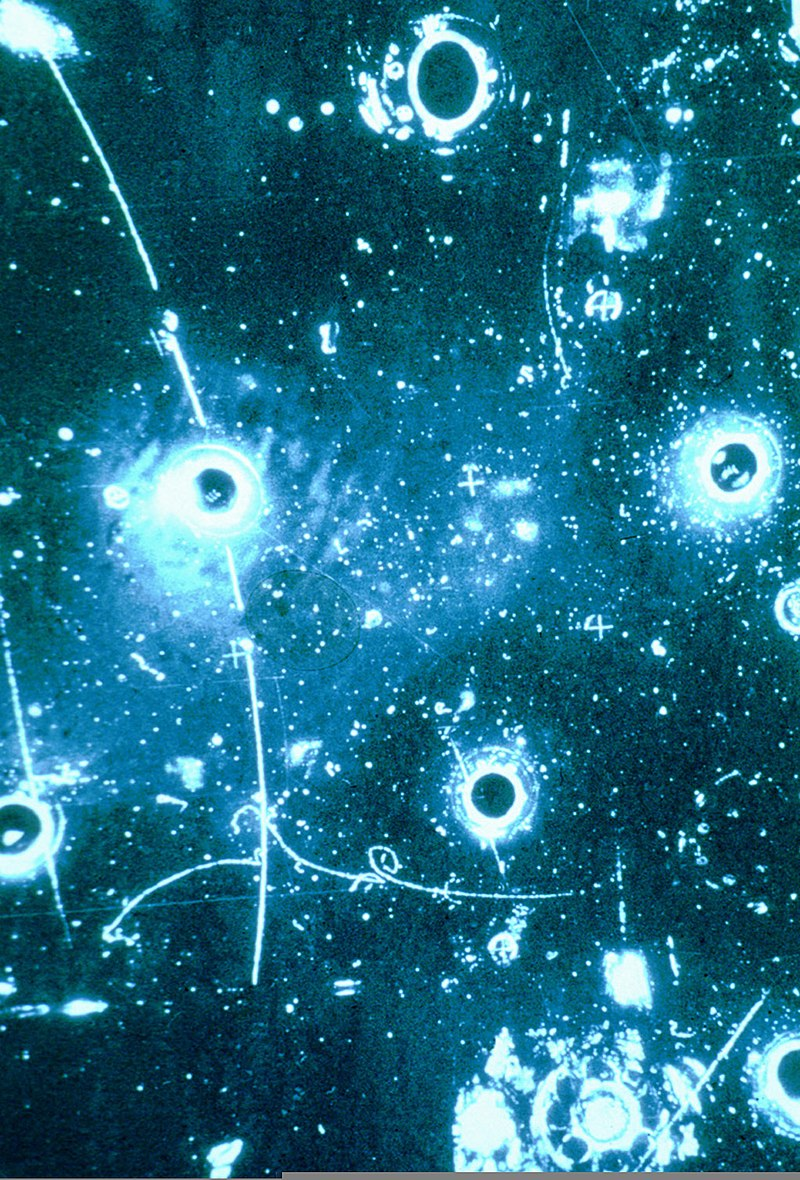
\includegraphics[width=4.5cm]{Leptonic_event_in_Gargamelle_bubble_chamber.jpg}}
\end{picture} \\ Doç. Dr. Mesut Karakoç}


\date{\today}

\begin{document}

%% Turkish babel problem
%% https://tex.stackexchange.com/questions/160385/newgeometry-doesnt-work-with-turkish-babel-package
%%\shorthandoff{=}% Make = not active any more

\maketitle

\newpage

% change name to "İçindekiler"
\renewcommand{\contentsname}{İçindekiler}
\tableofcontents{}

\listoffigures
 
\listoftables

\newpage

{
\hspace{.5\textwidth}
\begin{minipage}{.5\textwidth}
\raggedleft
If all this damned quantum jumps were really to stay, I should be
sorry I ever got involved with quantum theory.

—Erwin Schrödinger
\cite{book:Ficek}

%% Latince için
%% post iacturam quis non sapit!
%% Who is not wise after he has lost something?
%% https://quizlet.com/23756827/latin-proverbs-h-flash-cards/
\end{minipage}
}

\setcounter{section}{1} %% THIS WILL BE DELETED when all chapters merged!
\section{Dalga-Parçacık İkilemi ve Schrödinger Denklemi}

Kuantum fiziğinin doğum sürecini anlattığımız bir önceki bölümün içeriği genellikle \emph{Eski Kuantum Teorisi} olarak adlandırılır. Çünkü, gerçekleştirilen keşifleri açıklamak için  kullanılan veya ortaya konan kuralların tam olarak birbirleriyle sağlam bir bağlantısının olduğunu söylemek pek mümkün değildir. Daha iyi bir açıklama için ortaya konan ``Kuantum Mekaniği" iki defa keşfedilmiştir denebilir, ilki 1925'te matris mekaniği formalizmiyle Werner Heisenberg tarafından ve ikincisi 1926'da dalga mekaniği ile Erwin Schrödinger tarafındandır. Her ikisinin eş değer olduğu sonradan gösterilmiş olmasına rağmen Schröndinger'in yöntemi daha çok kullanılır hale gelmiştir. Çünkü dalga mekaniğinin matematiği fizikçiler arasında daha yaygındı \cite{book:Gasiorowicz}.


\subsection{Dalga-Parçacık İkilemi}
Kuantum fiziğini başlatan deneyler ve deneyleri açıklamak için geliştirilen teori ve modeller; klasik fizikte parçacık olarak bilinen (elektron, proton, nötron vb.) fiziksel varlıkların dalga özellikleri gösterdiklerini, benzeri şekilde dalga özelliği gösteren elektromanyetik dalganın parçacık (foton) özelliği gösterdiğini doğrulamıştır. 


\begin{figure}[hbtp]
\center

\includegraphics[scale=.5]{Wave-particle.png}
\caption{Işık bir dalgadır!?}
\label{fig:light_is_a_wave}
\end{figure}

Bu durumda kuantum fiziğinin sınırları içine giren herhangi bir fiziksel varlık, hem dalga hem de parçacık davranışı gösterebilmektedir. Dalga özelliği gösteriyorsa; kutuplanma, girişim ve kırınım gibi davranışlar göstermesi beklenirken, parçacık özelliği gösterdiğindeyse; klasik fizikteki gibi enerji ve momentum taşıması beklenmektedir. Belirli şartlar altında ışığın veya herhangi bir elektromanyetik dalganın enerji ve momentum taşıdıkları fotoelektrik etkisi, Compton saçılması ve karacisim ışıması deneylerinde göz1enmiştir.

Fakat her iki özelliğin de gözlenebiliyor olması öyle kolayca anlaşılamayabilir. Compton etkisi (veya saçılması) deneyiyle ışığın foton adı verilen bir parçacık gibi davrandığı doğrulanmıştır. İnsan gözüyle fotonlar tek tek seçilemese de, fotonları tek tek seçebilen ve fotoçoklayıcı \cite{book:Gasiorowicz} olarak adlandırılan cihazlar mevcuttur. 

Dirac'ın kuantum mekaniği üzerine yazdığı bir kitabında ilginç bir düşünce deneyi vardır. Belirli bir kutuplanmaya sahip ışık fotoelektrik etkide olduğu gibi elektron elde etmek için kullanılırsa, yayınlanan elektronların açısal dağılımı fotonların kutuplanmasıyla ilişkilidir. Fotoelektrik etkiye göre bir foton bir elektron koparabildiğine göre, fotonlar enerji ve momentuma ek olarak kutuplanmaya da sahiptir. Buna göre başlangıçta $I_0$ şiddetine sahip ve kutuplanmış bir ışık demetini sadece belli bir kutuplanma eksenindeki ışığın geçmesine izin veren bir kristalden geçirdiğimizi düşünelim. Eğer gelen ışığın tamamı kristalden geçecek kutuplanmaya sahipse geçen ışığın şiddeti de $I_0$ olacaktır. Eğer kutuplanma vektörü kristalin kutuplandırma ekseni ile $\theta$ açısı kadar farka sahipse, geçen ışık şiddeti $I_0 \cos^2 \theta$'a kadar olur. Bu durumu her bir foton için tek tek ele alalım. Eğer ışık demeti tamamen kristalin kutuplanma ekseni ile aynı yönde kutuplanmışsa demeti oluşturan bütün fotonların hepsi aynı yöndeki kutuplanmaya sahiptir. Fakat farklı bir polarizasyona (kutuplanmaya) sahip bir ışık demetinde ise demetin şiddeti  $\cos^2 \theta$ ile belirlenen oran kadar azalacaktır. Bunun anlamı bu oran kadar fotonun kristalden geçebilmesidir. Fakat, \emph{fotonlar bölünemezler} bu durumda bir foton kristalden ya geçer ya da geçemez. Bireysel olarak hangi fotonun geçtiğini bilmemiz mümkün değildir. Bütün söyleyebileceğimiz $N$ tane foton geldiyse, bunun $N \cos^2 \theta$ kadarının geçtiğidir. Böyle bir fotonun bu kristalden geçebilme olasılığı $\cos^2\theta$ olur.

Klasik optik fiziğine göre  bir çok foton içeren bir ışık demeti girişim ve kırınım gibi dalga özellikleri gösterecektir. Işığın dalga özelliğinin tek bir foton için de geçerli olduğunu gösteren bazı deneyler gerçekleştirilmiştir. Bunlardan birisi de G. I. Taylor tarafından 1909 yılında yapılmıştır. Bu deneyde bir iğne ucu etrafında çok düşük şiddetteki (bir kerede bir fotonun geçtiği) ışığın bile kırınıma uğradığı gösterilmiştir. Bu bize ışığın dalga davranışının fotonların toplu (kollektif) bir davranışı sonucunda değil de, bireysel özelliklerinin bir sonucu olarak var olduğunu göstermiştir. Bu durumda yeni sorunlar ortaya çıkmaktadır.


\begin{figure}[hbtp]
\center
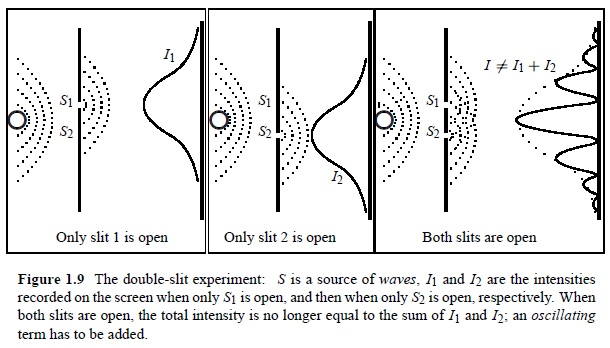
\includegraphics[scale=.8]{Double-slit_experiment_unknown_source.png}
\caption{Buraya benzeri bir başka şekil konacak!}
\label{fig:dobule_slit_experiment}
\end{figure}

Taylor'un deneyinin bir benzeri olan çift yarık deneyini düşünelim. Diğer deneydeki gibi her defasında bir foton gelsin ve Şekil \ref{fig:dobule_slit_experiment}'deki gibi yarıklardan birinden geçtikten sonra arkadaki ekranda yakalansın. Her iki yarıkta açıkken, yeterince sayıda foton geçtikten sonra klasik olarak beklendiği üzere (ışık dalga olduğundan) Şekil \ref{fig:dobule_slit_experiment}'in en solundaki gibi bir girişim deseni gözlenir. Klasik olarak bu durum çok rahat açıklanabilir. Eğer yarık 1 ve yarık 2'den geçen elektromanyetik dalgalar $\vec E_1(\vec r, t)$ ve $\vec E_2(\vec r, t)$ ile temsil edilirlerse, arkadaki ekrandaki bir $\vec r$ konumunda $t$ anında toplam dalga bu iki dalganın toplamı olacaktır. Bu klasik elektromanyetik teorinin bir parçası olan Maxwell denkleminin lineer olması dolayısıyla üst üste binme (süperposizyon) ilkesine uymasının sonucudur. Arkadaki ekranda gözlenecek olan ışığın toplam şiddeti ise,
%%
\begin{equation}
I \,\, \propto\,\, E^2 = \vec E \cdot \vec E = |\vec E_1 + \vec E_2|^2 = E_1^2 + E_2^2 + 2\vec E_1 \cdot \vec E_2
\label{eq:foton_interference}
\end{equation}
%%
denklemi ile belirlenir. Oluşan girişim deseninin matematiksel kaynağı $\vec E_1 \cdot \vec E_2$'dir. Eğer iki yarıktan sadece birisi açık olsaydı, sadece $|\vec E_1|^2$ veya $|\vec E_2|^2$ ile orantılı şiddetler gözlenebilirdi. Eğer bu şiddetleri polarizasyon deneyinde olduğu gibi olasıkla ilişkilendirirsek, sadece birinci veya ikinci yarıktan geçme olasılıkları sırasıyla $P_1(r,t)$ ve $P_2(r,t)$ olurken, her iki delik açıkken geçme olasılıkları bu iki olasılığın doğrudan toplamı olmaz.

Fotonlar bölünemez olduklarına göre ve bu davranış tek bir foton için de geçerli olduğuna göre, bu durum ancak \emph{bir fotonun kendi kendisiyle girişim} yapabileceğini varsaymakla çözülebilir. Böyle bir fotonun iki yarıktan açıkken sahip olacağı klasik elektromanyetik dalga alanı,
%%
\begin{equation}
\vec e = \vec e_1 + \vec e_2
\label{eq:single_foton_em_field}
\end{equation}
%%
şeklinde olacaktır ve Maxwell'in çizgisel klasik elektromanyetik dalga denklemlerine uygun olacaktır. Polarizasyon deneyinde olduğu gibi bu deneyde de tek bir fotonun hangi yarıktan geçtiğini bilmek mümkün değildir.


İlk keşfedildiklerinde elektronların parçacık yönüyle karşılaşılmıştır. Klasik olarak hareketlerinin yörüngesi üzerlerine etki eden manyetik ve elektrik alanlar ile belirlenebilir, kütlelidirler, enerji ve momentum taşırlar. Daha sonraları elektron kırınımı ve elektron için çift yarık deneyleriyle elektronların da dalga davranışı gösterdikleri gösterilmiştir. Elektron için gerçekleştirilen çift yarık deneyinde de, yukarıda foton için gerçekleştirdiğimiz düşünce deneyine benzer şekilde, elektronların çift yarıktan geçtikten sonra arkadaki ekranda girişim desenleri oluşturdukları gözlenmiştir. Fotonlarda girişim deseninin oluşma nedeni toplu bir davranışın değil bireysel davranışların sonucuydu, elektronların girişim deseni de aynı şekilde bireysel bir davranışın bir sonucudur. Foton için tanımladığımız gibi elektronun kendi kendisiyle girişimini ifade eden bir dalga fonksiyonu tanımlamak mümkündür. Böylece çift yarık deneyindeki bir elektronun dalga fonksiyonu,
%%
\begin{equation}
\psi(\vec r, t) = \psi_1(\vec r, t) + \psi_2(\vec r, t)
\label{eq:single_electron_wave}
\end{equation}
%%
olarak yazılabilir. Bu dalga fonksiyonunun elektronun girşimini izah eden çizgisel bir denkleme uyması beklenir. Böylece elektronun yarıklardan birisi açık olduğundaki dalga fonksiyonlarının toplamı, üst üste binme ilkesi gereğince, her iki yarık açık olduğundaki dalga fonksiyonunu vermelidir. Böyle bir dalga fonksiyonunu kullanan ünlü bir çizigisel denklem {\bf Schrödinger denklemi}'dir. Bu denklemde $\psi (\vec r, t)$ elektronun $\vec r$ konumunda ve $t$ anında ikinci ekranda bulunma olasılığıyla ilişkilidir. 

\subsection{Düzlem Dalgalar ve Dalga Paketleri}

Bu bölümde sıradan düzlem dalgalardan yola çıkarak elektron gibi bir parçacığın parçacık özelliklerini de içerecek olan \emph{dalga paketi} kavramını incelyeceğiz. Bu dalga paketleri parçacıkları temsil etmekle beraber, sanki gerçekten parçacık gibi davranan dalga paketleri varmış gibi düşünmek doğru değildir \cite{book:Gasiorowicz}.

Basit harmonik bir hareketi tanımlayan $k$ dalga sayısına sahip ve $+x$ yönünde ilerleyen bir dalga,
%%
\begin{equation}
\psi_k(x, t) = A_1 \cos(kx - \omega t) + A_2 \sin(kx - \omega t)
\label{eq:plane_sin_wave}
\end{equation}
%%
olarak veya,
%%
\begin{equation}
\psi_k(x, t) = A \text{e}^{i(kx - \omega t)} + B \text{e}^{-i(kx - \omega t)}
\label{eq:plane_exp_wave}
\end{equation}
%%
şeklinde yazılabilir. Dalga sayısı ve dalga boyu arasında, açısal frekans ve periyot arasında ve açısal frekans ile frekans arasında sırasıyla aşağıdaki bağıntılar vardır;
%%
\begin{equation}
k = 2\pi/\lambda, \,\,\,\, \omega = 2\pi/T,\,\,\, \text{ve}\,\,\, \omega = 2\pi\nu.
\label{eq:wave_length_number}
\end{equation}
%%
Klasik dalgalardan hatırlanacağı üzere $\omega$ ve $k$ arasındaki bağıntı, bir dalganın dağınımlı bir ortamda mı, yoksa dağınımsız bir ortamda mı ilerlediğiniz belirlemektedir. Örneğin boşlukta ilerleyen ışık (veya elektromanyetik dalga) için $\omega$ ve $k$ arasındaki bağıntı,
%%
\begin{equation}
\omega = 2\pi \nu = 2 \pi c/\lambda \text{, olduğundan }\, \omega = c k
\label{eq:w_k_relation}
\end{equation}
%%
olur. Çünkü dağınımsız ortamlarda $\omega$ ve $k$ doğru orantılıdır. Dağınımlı bir ortam da ise açısal frekans dalga sayısının ($\omega(k)$) bir fonksiyonu olarak yazılabilir. Örneğin, dağınımlı ortamda ışığın frekansı ortamın kırılım indeksine bağlı olarak $\nu = c/n\lambda$ şeklinde yazılabilir. $n$ ise genellikle $\lambda$'nın bir fonksiyonudur. Doğal olarak $\omega$ ve $k$ arasındaki doğru orantının kaybolacağı açıktır.
%%
\begin{figure}[hbtp]
\center
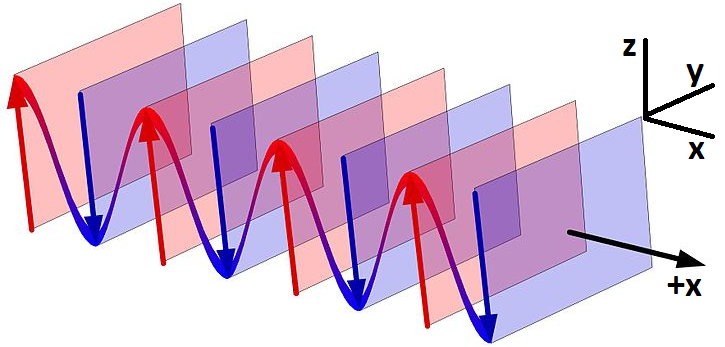
\includegraphics[scale=1.5]{Plane_Wave_Oblique_View.png}
\caption{$+x$ yönünde ilerleyen ve $y-z$ düzleminde sabit değerli olan düzlem dalganın temsili çizimi.}
\label{fig:plane_wave}
\end{figure}
%%
%%
Şimdi yukarıdaki bilgilere göre dalga paketi kavramını tanımlaya çalışalım. $\psi_k(x,t)$ $y$ ve $z$'den bağımsız olduğu için Şekil \ref{fig:plane_wave}'deki gibi bir davranışa sahip düzlem dalgadır. $\psi_k(x,t)$ ile bir kuantum davranışlı varlığın (elektron, foton v.b.) bütün sahip olabileceği $k$ değerli dalga fonksiyonlarını tanımlamak mümkündür. Çift yarık deneyinde elektron veya foton için sadece iki dalga fonksiyonunun süperpozisyonu söz konusuyken bu durumda bütün olası durumları göz önüne alabilmek için genliği $k$'ye bağlı $A(k)$ genlikli,
%%
\begin{equation}
\psi_k(x, t) = A(k) \text{e}^{i(kx - \omega t)} 
\label{eq:plane_wave_A_k}
\end{equation}
%%
bir ilerleyen düzlem dalga yazmak mümkündür. Bu düzlem dalgaların süperpozisyonu ise,
%%
\begin{equation}
\psi(x, t) \equiv \int\limits_{-\infty}^{\infty}dk\,\psi_k(x, t) = \int\limits_{-\infty}^{\infty}dk\,A(k) \text{e}^{i(kx - \omega t)} 
\label{eq:wave_packet}
\end{equation}
%%
ile elde edilir. Süperpozisyon sonucu elde edilen bu dalga fonksiyonu, \emph{dalga paketi} olarak adlandırılır. Dalga paketi $t=0$'da
%%
\begin{equation}
\psi(x, 0) = \int\limits_{-\infty}^{\infty}dk\,A(k) \text{e}^{i(kx)} 
\label{eq:wave_packet_t0_int}
\end{equation}
%%
olur. Klasik parçacıklar dalgalardan farklı olarak belirli bir konuma sahip olduklarından ve bir dalga paketi ile parçacık özelliklerini tanımlamak istediğimizden, dalga paketinin erişimi de sonlu bir dağılım olmalıdır. Bu nedenle $A(k)$,
%%
\begin{figure}[hbtp]
\center
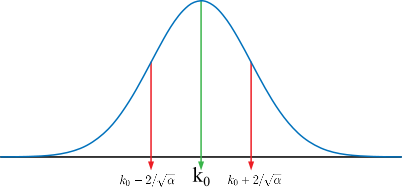
\includegraphics[scale=1.5]{Gaussian_distribution.png}
\end{figure}
%%
\begin{equation}
A(k) = \text{e}^{-\alpha (k-k_0)^2/2}
\label{eq:wave_packet_t0}
\end{equation}
%%
gibi, gausyen (gaussian) dağılım olarak adlandırılan, bir dağılım tercih edilebilir. Bu dağılımın merkezi $k_0$ civarındadır ve merkezden uzaklaşırken hızlıca değeri azalır. Daha sonra bir parçacığın momentumunun belirli bir aralıkta olma özelliğini tanımlayan bu fonksiyonun karesinin önemli olduğunu göreceğiz. Kare fonksiyonun tepe değerinden $\frac{1}{3}$ değerine $\alpha (k-k_0)^2\eqsim 1$ civarında düşer. Buna göre bu dağılımın genişliği $\Delta k \equiv = k-k_0 = 2/\sqrt{\alpha}$ olarak tanımlanabilir. $t=0$'daki dalga paketini tanımlayan integral önce $q' = k-k_0$ değişken dönüşümü yapılarak,
%%
\begin{equation}
\psi(x, 0) = \text{e}^{ik_0x} \text{e}^{x^2/2\alpha} \int\limits_{-\infty}^{\infty}dq' \, \text{e}^{-\alpha q'^2/2} = \sqrt{\frac{2\pi}{\alpha}} \text{e}^{ik_0x} \text{e}^{x^2/2\alpha}
\label{eq:wave_packet_t0}
\end{equation}
%%
şeklinde çözümlenebilir. Sabitleri göz önüne almazsak elde ettiğimiz dalga paketi sanki yeni bir dağılım fonksiyonuyla düzlem dalganın çarpımı gibi durmaktadır. Bu yeni dağılım fonksiyonu parçacığı $x=0$ civarında yerelleştirmeye çalışmaktadır. $A(k)$ dağılım fonksiyonuna benzer şekilde bu dağılım fonksiyonun genişliği ise $\Delta x \equiv  x - 0 = 2\sqrt{\alpha}$'dır. İlginç bir şekilde dalga paketinin şeklini belirleyen $\Delta k$ ve $\Delta x$ genişliklerinin çarpımı,
%%
\begin{equation}
\Delta k  \Delta x  = 4
\label{eq:del_x_k}
\end{equation}
%%
değerine sahiptir ve $\alpha$'dan bağımsızdır. Bu ilişki Fourier türü integrallerin genel bir özelliğidir.


Bir dalga paketinin $t=0$ anında sahip olabileceği formunu ve bu formun genişliğini sınırlayan bir bağıntı elde etmiş olduk. Bu dalga paketinin zamanla nasıl ilerleyeceğini ise (şimdilik) yaklaşık olarak çalışmak yeterlidir. Bu yaklaşıklıkta $k_0$ etrafında çok dar bir dağılıma sahip bir dalga paketini düşünelim, böyle bir dağılım için çok geniş bir $x$ dağılımına sahip olacaktır. Bu özelliklere sahip dalga paketi aşağıdaki gibi tanımlanan grup hızı ile hareket eder (\href{https://www.youtube.com/watch?annotation_id=annotation_1566711117&feature=iv&src_vid=MMV2Zt7x430&v=v9DPzMoWpc0
}{grup hızını ve faz hızını karşılaştıran bir video bağlantısı}).
%%
\begin{equation}
v_g = \frac{\partial \omega(k)}{\partial k} \bigg |_{k=k_0}
\label{eq:group_velocity}
\end{equation}
%%
Denk. \ref{eq:wave_packet}'e göre $A(k)$ ve $\omega(k)$'nın davranışı bilinirse dalga paketinin zamanla değişimi hakkında bilgi sahibi olunabilir. Dalga paketi$k_0$ etrafında dar bir dağılıma sahip olduğundan $A(k)$ çok keskin artan bir tepe şeklinde olacaktır. $\omega(k)$'nın ise $k$'nın yavaş değişen bir fonksiyonu olduğunu kabul edersek $\omega$ için yaklaşık olarak,
%%
\begin{equation}
\omega(k) \eqsim \omega(k_0) +  (k-k_0) \frac{\partial \omega(k)}{\partial k} \bigg |_{k=k_0} + \frac{1}{2}(k-k_0)^2 \frac{\partial^2 \omega(k)}{\partial k^2} \bigg |_{k=k_0}  
\end{equation}
ifadesi yazılabilir. Böylece $(kx-\omega t)$ için de,
%%
\begin{equation*}
(kx - \omega(k)t) \eqsim (k_0 x - t \omega(k_0)) +  (k-k_0)\left[x - t\frac{\partial \omega(k)}{\partial k} \bigg |_{k=k_0} \right] - \frac{t}{2}(k-k_0)^2 \frac{\partial^2 \omega(k)}{\partial k^2} \bigg |_{k=k_0}  
\end{equation*}
eşitliği elde edilir. Bu ifade Denk. \ref{eq:wave_packet}'te yerine konursa ve $q=k-k_0$ değişken dönüşümü yapılırsa,
\begin{equation}
\psi(x, t) \eqsim  \text{e}^{i(k_0x - \omega(k_0) t)}  \int\limits_{-\infty}^{\infty}dq\,A(q + k_0) \text{e}^{iq(x - v_g t)} \text{e}^{-iq^2\beta t/2} 
\label{eq:wave_packet_t_change}
\end{equation}
dalga paketi integraline ulaşılır, burada $\beta$ sembolü
\begin{equation*}
\beta = \frac{\partial^2 \omega(k)}{\partial k^2}\bigg |_{k=k_0}
\end{equation*}
olarak integrali kısaltmak için tercih edilmiştir.


\newpage
% In the preamble, add "\renewcommand\refname{New Title}" for article type documents 
% and "\renewcommand\bibname{New Title}" for book and report type documents.
\renewcommand\refname{Kaynaklar}
\bibliography{quantumBIB}{}
%% https://www.sharelatex.com/learn/latex/bibtex_bibliography_styles
 \bibliographystyle{plain}
%% \bibliographystyle{alpha}
%%\bibliographystyle{apalike}
\end{document}

